% !TeX root = ../thuthesis-example.tex

\chapter{三维面部和骨骼模型的重建}
\label{cha:reconstruction}

精确和高效的正颌外科手术模拟,其先决条件是从医疗成像数据中准确重建出三维的面部与骨骼模型。
本章详尽地阐述了该三维模型重建的方法和流程,具体内容包括:
\begin{enumerate}
  \item 提取 CT 图像数据以形成面部与骨骼表面模型的三角网格表示,
  \item 对模板模型与患者模型进行刚性配准,
  \item 采用非刚性配准对模板模型进行形变,以更精确地匹配骨骼和表面的形状,
  \item 对模型表面进行体积细分,以构建模拟患者软组织的四面体网格。
\end{enumerate}
经过以上步骤,我们能够生成手术前后拓扑基本一致的三角网格模型,并且将该模型划分为高质量的四面体网格。

本文所采用的 CT 数据分辨率为 \numproduct{512 x 512 x 364} 体素,每个体素的尺寸为 \qtyproduct{0.4395 x 0.4395 x 0.6000}{\milli\meter}。

\section{模板模型的构建}

为满足本研究的需求,我们以 SCULPTOR \cite{qiuSCULPTORSkeletonconsistentFace2022a} 开源的骨骼及面部模板为基础,构筑了所需的模板模型。
初始阶段,我们手动移除 SCULPTOR 模板中的非必要部分,如颈部和复杂的口唇区域。
随后,利用 MeshFix 工具 \cite{atteneLightweightApproachRepairing2010} 填补了模板中的空洞,这些空洞主要位于眼部、口部以及颈部的精细区域,并解决了因自相交缺陷导致的穿模问题。
最后,我们对模型应用了 Taubin 平滑 \cite{vollmerImprovedLaplacianSmoothing1999},以降低模型中的锐利缺陷。

\section{刚性配准}

本节主要讲述如何从 CT 体素数据提取三角网格表面模型,并进行模型之间的刚性配准。

首先,我们对体素数据施加 Gaussian 平滑处理,以滤除 CT 扫描中由散射和噪声所引入的过锐缺陷。
之后,按照预设阈值对 CT 值进行分割,并使用 VTK Contour Filter 方法提取骨骼和面部的等值面,其中骨骼和软组织的 CT 阈值分别设置为 \num{200} 和 \num{-200}。

进一步,在模板和患者的三维模型的骨骼表面上分别标定了若干特征点,如图 \ref{fig:landmarks} 所展示的 10 个和 9 个特征点。
该步骤的目标是在模板与患者间建立精确的一对一特征点映射关系。

\begin{figure}
  \centering
  \subcaptionbox{10 个面部特征点\label{fig:landmarks-face}}{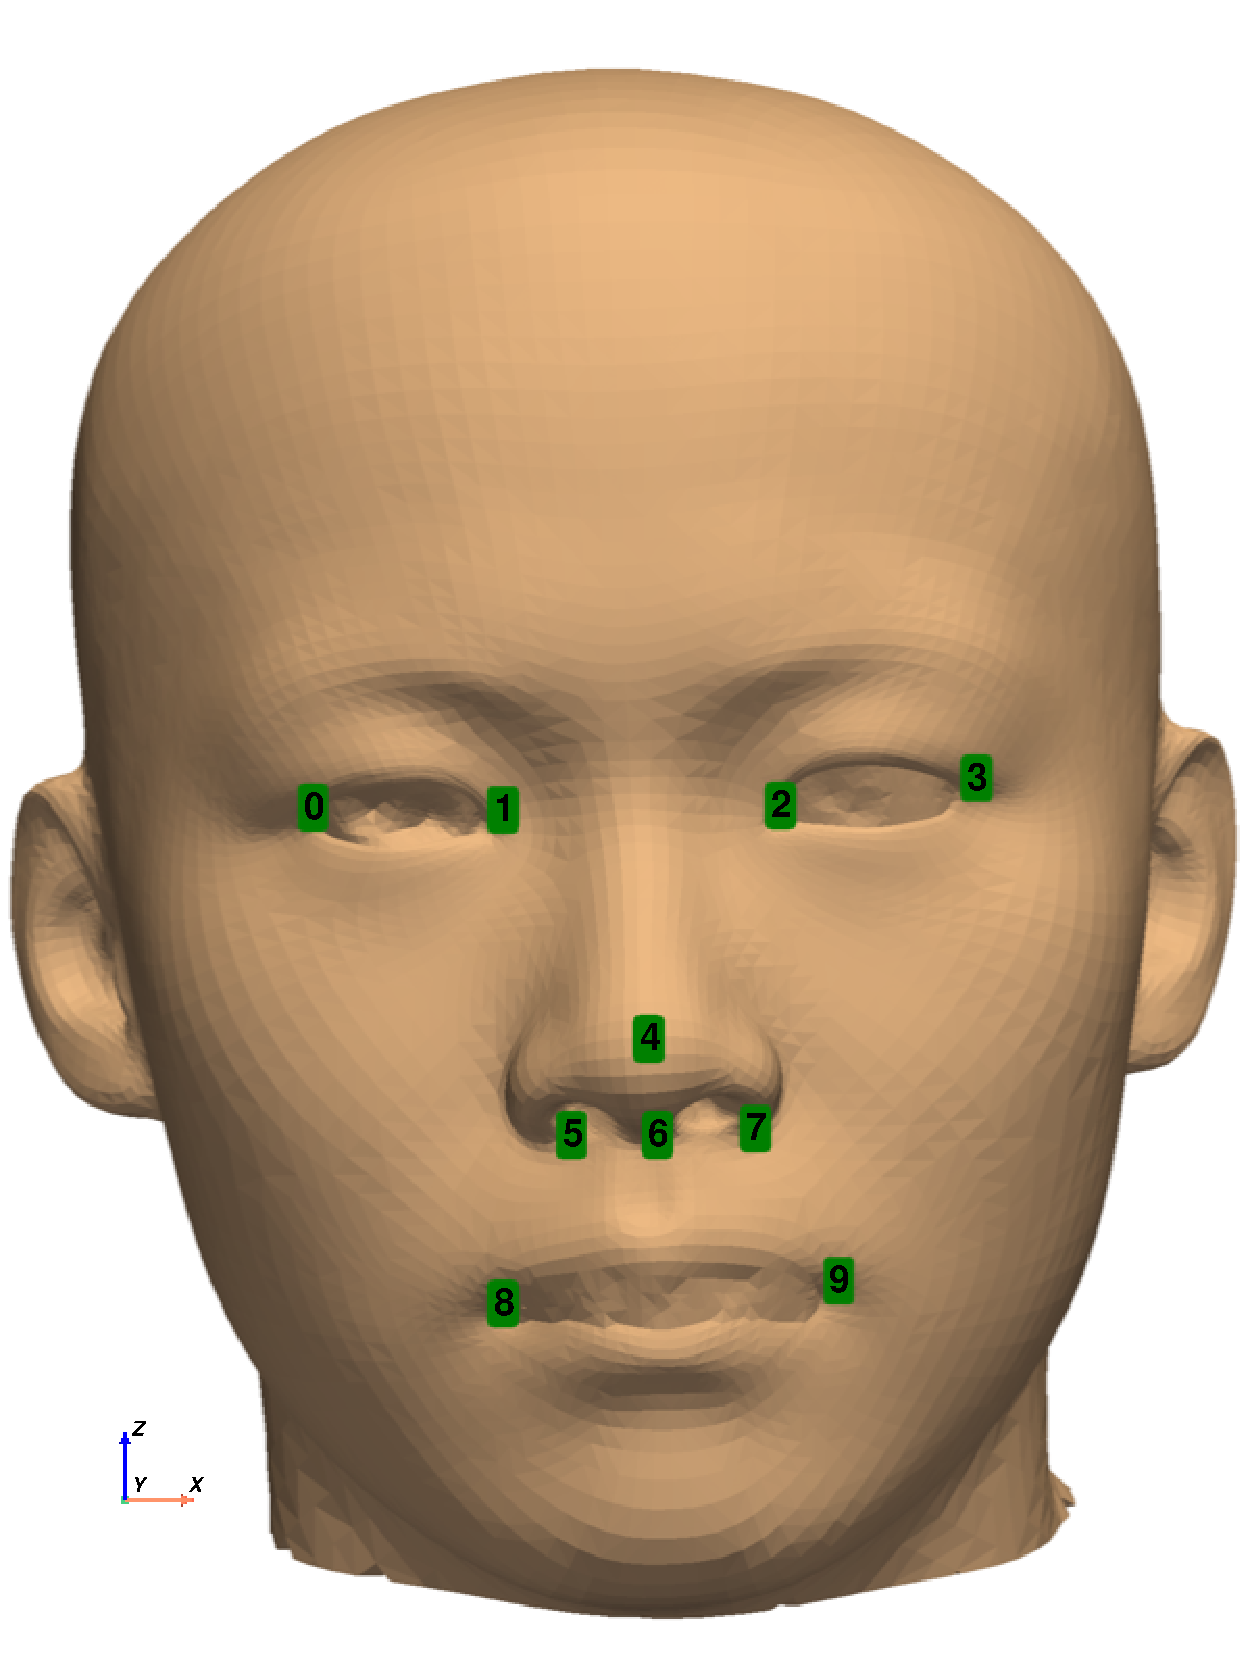
\includegraphics[width = 0.3 \linewidth]{landmarks/face-landmarks.pdf}}
  \subcaptionbox{9 个骨骼特征点\label{fig:landmarks-skull}}{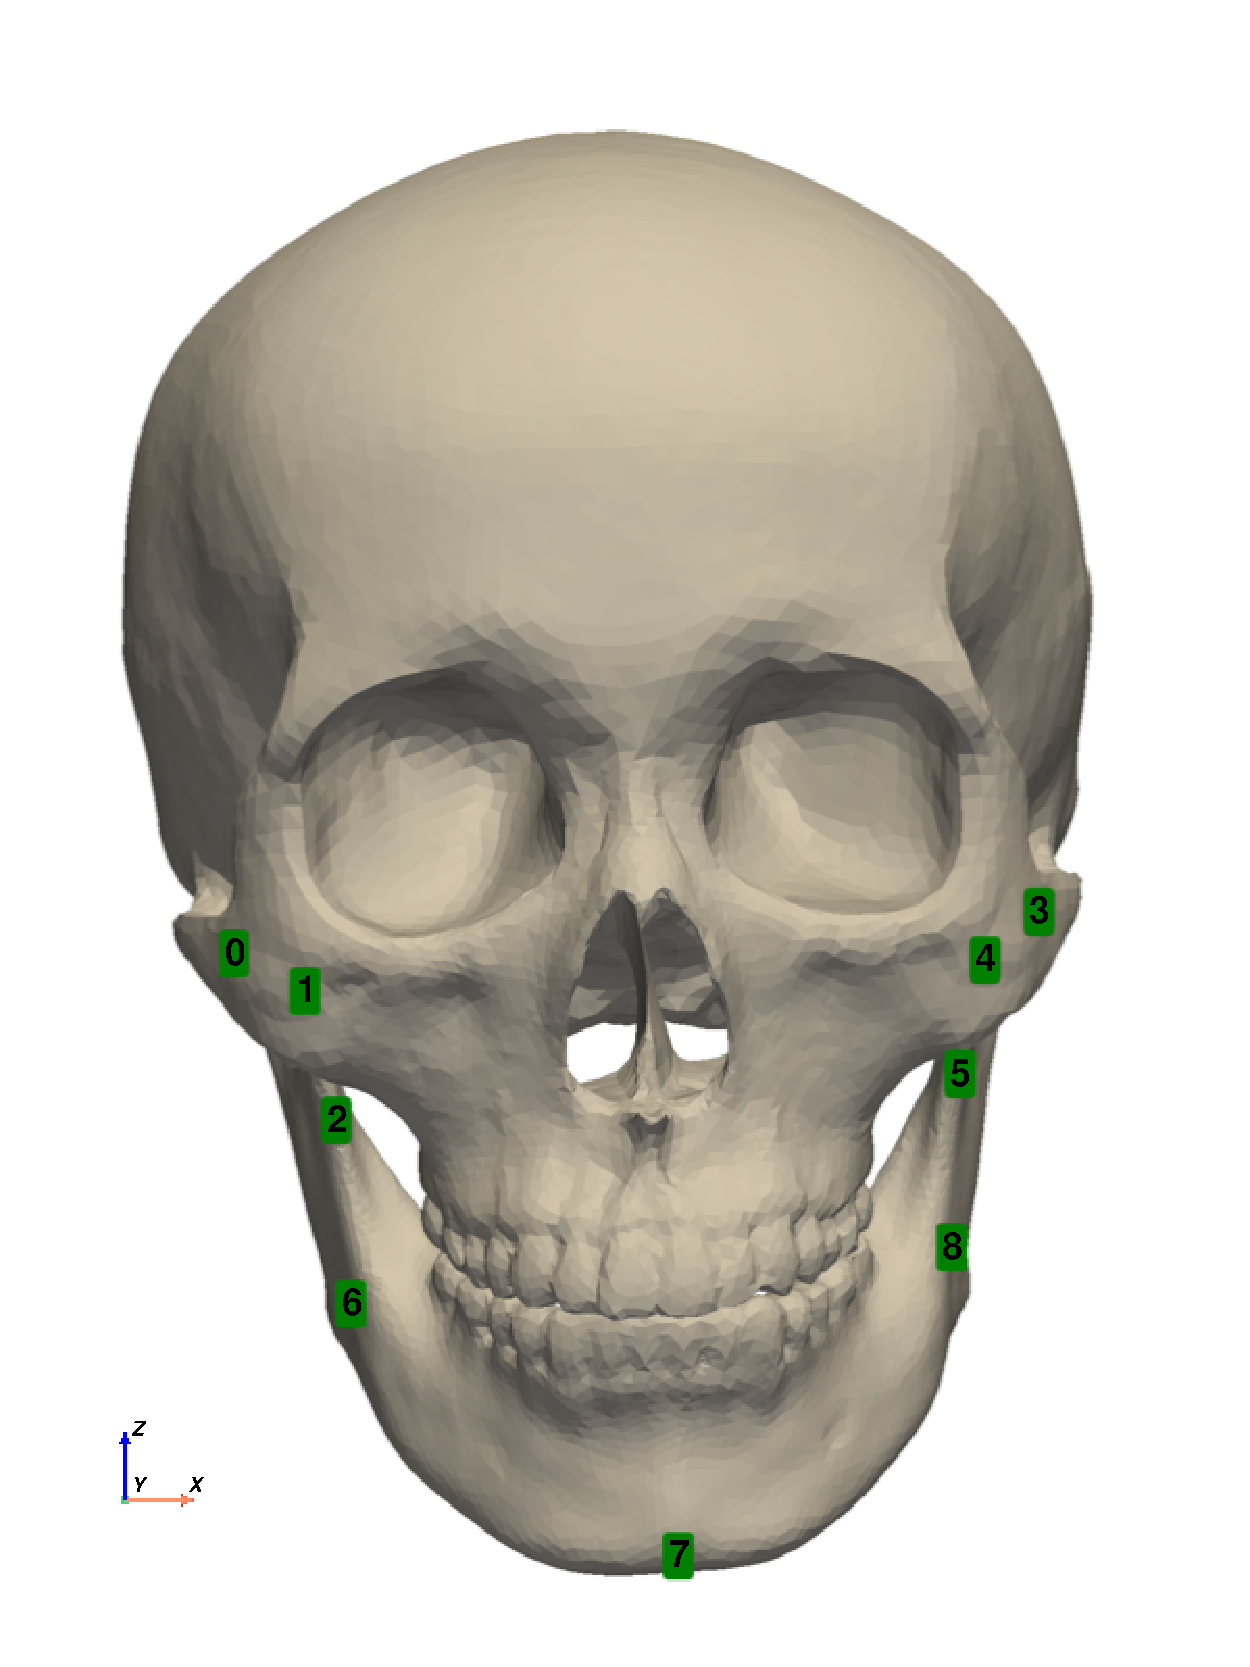
\includegraphics[width = 0.3 \linewidth]{landmarks/skull-landmarks.pdf}}
  \caption{特征点}
  \label{fig:landmarks}
\end{figure}

为了获得一组初始的刚性变换参数,即全局的平移、缩放与旋转参数,本研究采纳了标准的 Procrustes 分析方法 \cite{rossProcrustesAnalysis2004}。
Procrustes 分析的核心目标在于通过反复迭代的过程,最小化两组特征点之间的总平方距离。
在此基础之上,本研究进一步引入了迭代最近点(Iterative Closest Point,ICP)算法,对模型进行精细的刚性配准。
该步骤的主要目的在于减小由人工标注特征点过程中可能产生的误差。
具体的刚性配准结果如图 \ref{fig:align} 所展示。
值得注意的是,CT 数据往往具有相近的空间位态,因此对于多组 CT 扫描,我们可以通过单次 Procrustes 分析为所有模型建立一个相同的初始变换参数,再通过 ICP 算法进行进一步的提升配准的精度。

\begin{figure}
  \centering
  \subcaptionbox{面部}{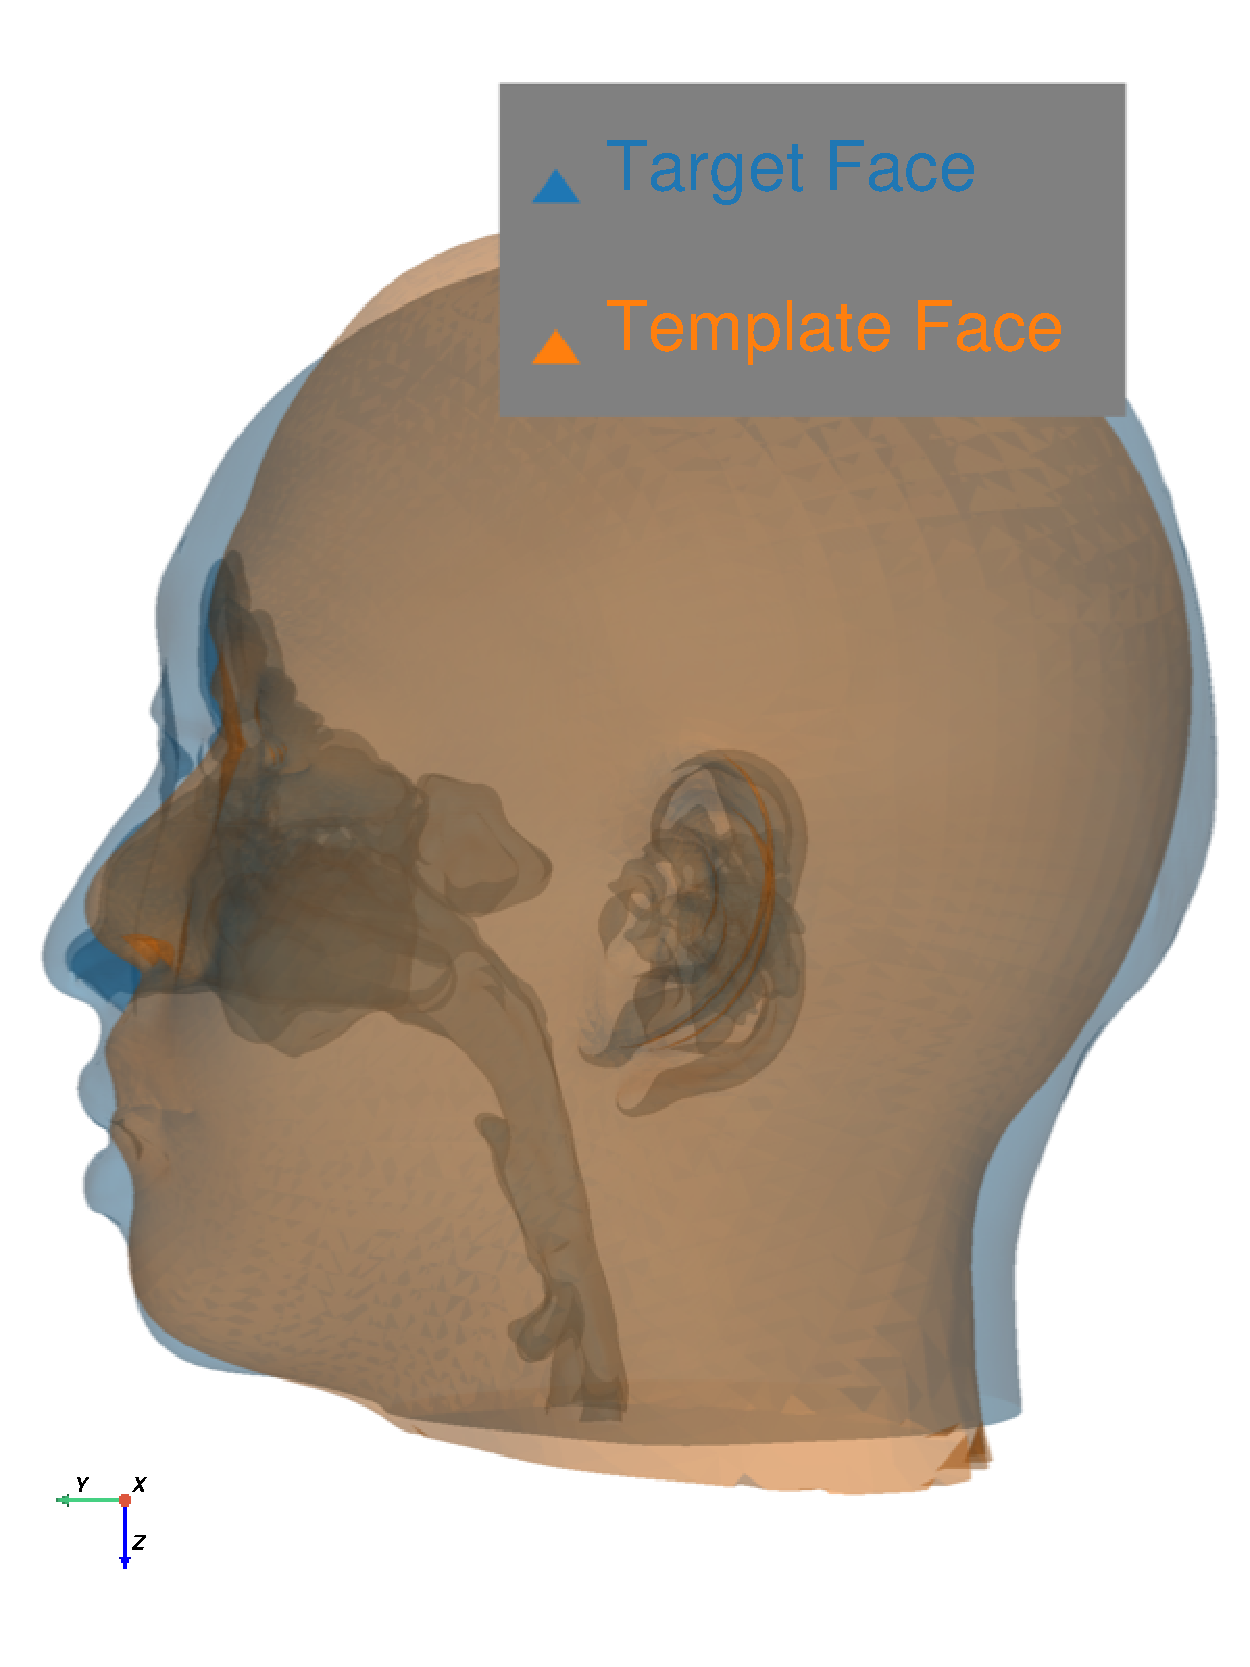
\includegraphics[width = 0.3 \linewidth]{align/align-face.pdf}}
  \subcaptionbox{骨骼}{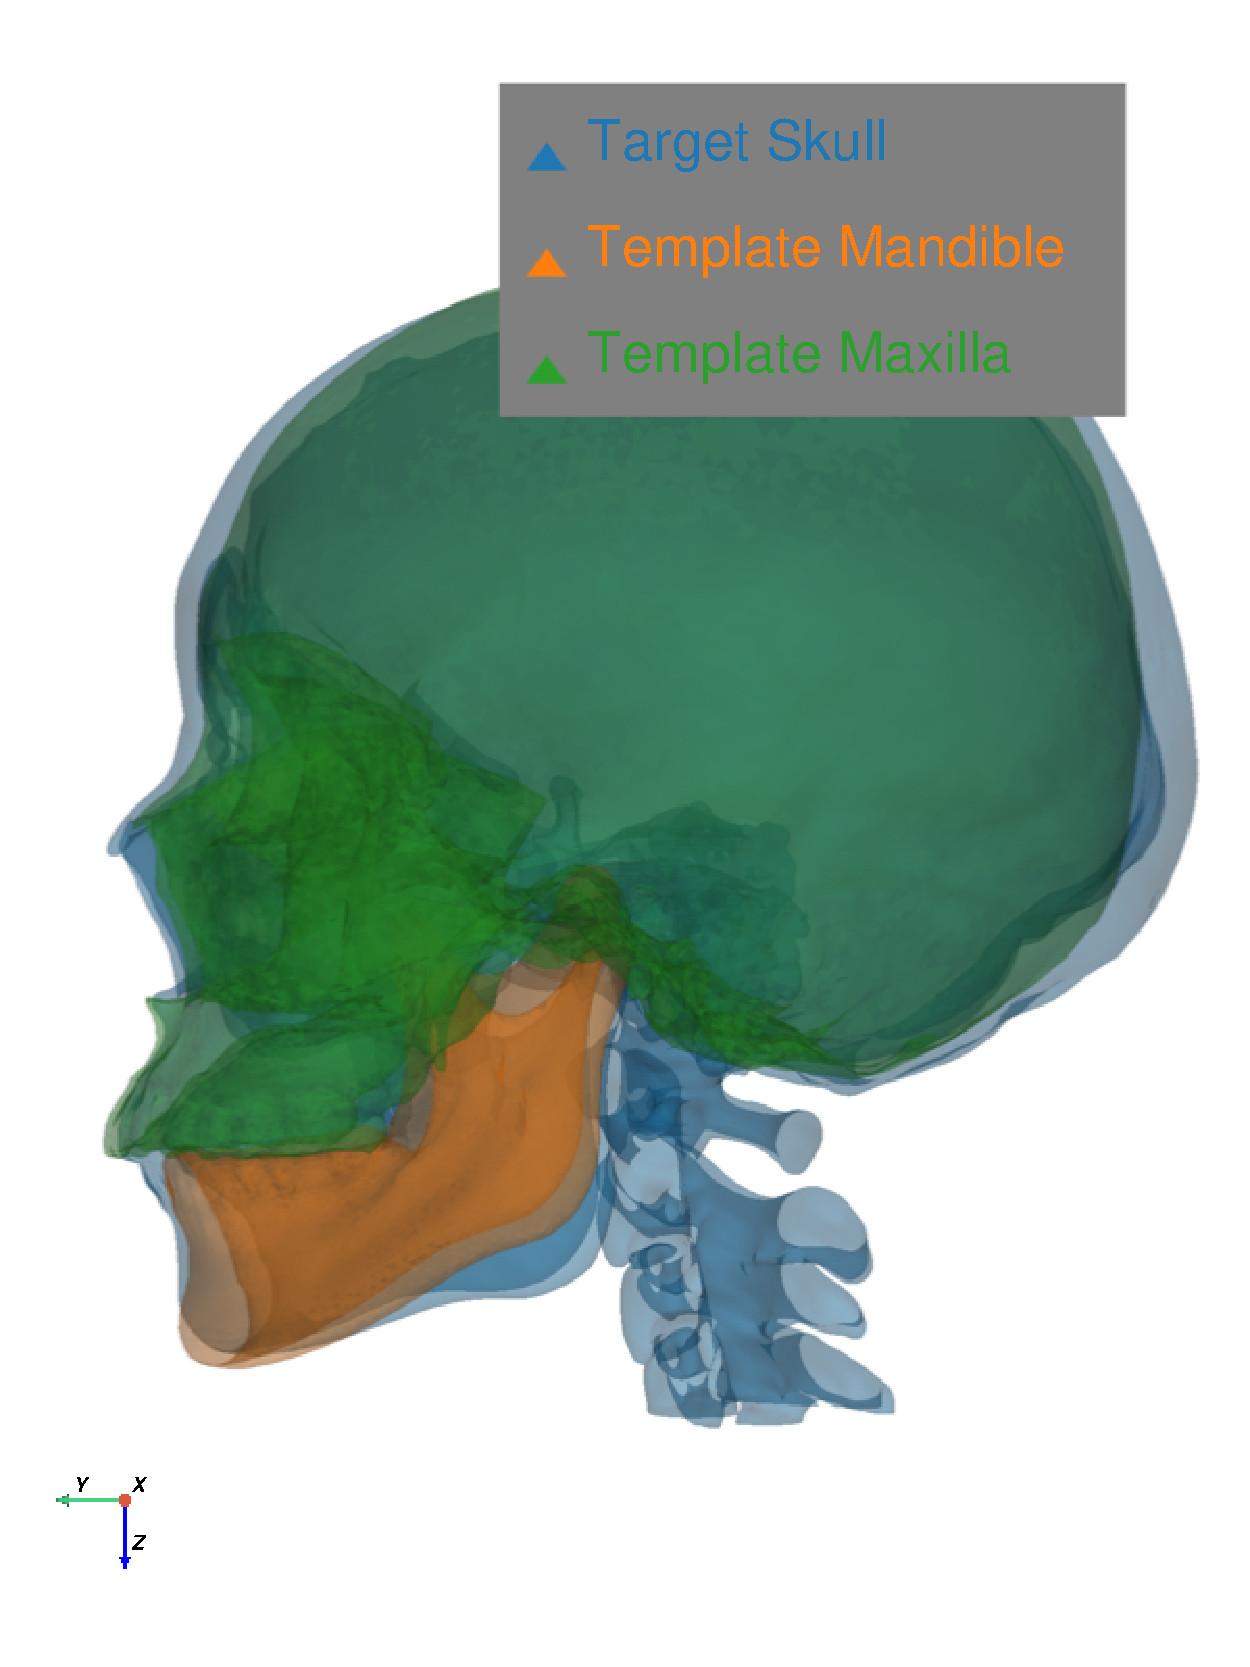
\includegraphics[width = 0.3 \linewidth]{align/align-skull.pdf}}
  \caption{刚性配准结果}
  \label{fig:align}
\end{figure}

\section{非刚性配准}

在完成了初始的刚性配准工作后,我们需要进行非刚性配准(non-rigid registration),以将模板模型变形至与患者一致。
我们采用了由 Amberg 等人提出的非刚性配准算法 \cite{ambergOptimalStepNonrigid2007} 作为理基础。
该算法将 ICP 扩展至非刚性形变来使模型与目标几何匹配。
在初始阶段,通过使用最邻近点来建立模板与目标患者模型间顶点的对应关系。
继而,该算法通过最小化能量函数 $E$ 来解算每个顶点的变换矩阵 $\bm{X}_i$。
在迭代过程中,对应关系与变换矩阵的交替进行更新,随着迭代次数的增加,对应关系趋于更为精确,引导变换矩阵的优化结果逐渐接近理想状态。

\subsection{对应关系的建立}

在考虑模板与患者模型之间的区域差异,例如,患者模型的面部部分相比模板多出口腔等区域,而其骨骼结构又包括额外的脊椎但不包含牙齿咬合面等细节。
由此,我们必须从两者中抽取交集区域,亦即重叠区域。
首先,我们对模板进行标注,标记出重叠区域 $\mathcal{S}_o$。
接着,可以根据下式确定患者模型的重叠区域 $\mathcal{T}_o$:
\begin{equation}
  \mathcal{T}_o = \Bqty{\bm{u}_i \mid \dist(\mathcal{S}_o, \bm{u}_i) < \tau, \bm{u}_i \in \mathcal{T}}
\end{equation}
其中,$\tau$ 代表预设的阈值。
在实际操作中,我们将 $\tau$ 设为对应患者模型边界框的对角线长度的 \SI{5}{\percent}。
从同一成像设备获取的 CT 数据中,重叠区域在空间范围上具有相似性。
因此,处理多组数据时,仅需对模板的重叠区域进行一次标注,再将该标注信息应用于其他患者模型即可。
这大大节省了时间和人力资源。

简单地采用最近邻顶点法进行初始化对应关系可能导致模板与患者模型之间的对齐不够精确。
例如,在下颌骨较为扁平的区域,最近邻顶点法可能会受限于狭窄空间,使得无法有效地将模板中的顶点与患者模型中的顶点匹配起来。
为了克服这一限制,在初始化对应关系时,我们加入了顶点法线作为额外的依据变量:
\begin{equation}
  \mathrm{NN}(\bm{v}_i) = \argmin_{\bm{u}_j \in \mathcal{T}_o} \norm{\bm{v}_i - \bm{u}_j}^2 + \nu \norm{\bm{n}_i - \bm{n}_j}^2
\end{equation}
式中,$\mathrm{NN}(\bm{v}_i)$ 表示模板顶点 $\bm{v}_i$ 在患者模型中的最近邻对应点,$\bm{n}_i$ 和 $\bm{n}_j$ 分别为模板顶点 $\bm{v}_i$ 与患者模型对应顶点 $\bm{u}_j$ 的法向量,而 $\nu$ 是一个超参数,用于调整法线在匹配过程中的权重。
我们利用 $k$-d 树(其中 $k = 6$)加速最近邻关系的搜索过程,此算法使得我们能够以 $\mathcal{O}(n \log{m})$ 时间复杂度完成所有顶点对应关系的确定,其中 $n$ 表示模板顶点的数量,$m$ 表示患者模型顶点的数量。
这种方法同样适用于求解反向对应关系。

\subsection{损失函数}

我们考虑一个包含 $n$ 个顶点的模板,其顶点集定义为 $\mathcal{S} = \{\bm{v}_i\}$,并且在模板上规定了一个重叠区域 $\mathcal{S}_o$。
我们的目标是识别一种逐顶点变换 $\mathcal{X}$,以便使得模板的重叠区域 $\mathcal{S}_o$ 能够适当变形以匹配到患者模型 $\mathcal{T}_o$ 上。
因此,我们将每个顶点的变换建模为一个包含平移和相对于模型中心旋转,数学上表达为:
\begin{equation}
  \bm{v}_i' = \bm{X}_i \bm{v}_i
\end{equation}
这里,$\bm{X}_i \in \mathbb{R}^{3 \times 4}$ 表征了第 $i$ 个顶点所受的仿射变换矩阵,$\bm{v}_i = [x_i ~ y_i ~ z_i ~ 1]^T$ 则表示顶点的齐次坐标。

为了高效衡量模板与患者模型间的误差,我们采用了一个混合损失函数,该损失函数由距离项、刚度项和特征点项组成,用以作为模板与患者模型间差异的评估指标。

\paragraph{距离项}
该项的目的在于实现模板顶点向患者模型顶点的尽量准确对齐。
为达至此目标,我们定义了顶点距离损失函数如下:
\begin{equation}
  E_d(\mathcal{X}) = \sum_{\bm{v}_i \in \mathcal{S}_o} w_i \dist^2(\mathcal{T}_o, \bm{X}_i \bm{v}_i)
\end{equation}
其中,权重 $w_i$ 由模板顶点 $\bm{v}_i$ 的法向量 $\bm{n}_i$ 以及患者模型中对应顶点 $\bm{u}_j$ 的法向量 $\bm{n}_j$ 之间的点积所决定,即 $w_i = \bm{n}_i \cdot \bm{n}_j$。

\paragraph{刚度项}
在形变匹配的同时保持模板的原有刚性特性是极其重要的。
鉴于此,我们引入刚度项 $E_s$ 来度量此种特性。
刚度项的定义如下:
\begin{equation}
  E_s(\mathcal{X}) = \sum_{(\bm{v}_i, \bm{v}_j) \in \mathcal{E}} \norm{(\bm{X}_i - \bm{X}_j) \bm{G}}_F^2
\end{equation}
此处,$\mathcal{E}$ 代表模板中所有边的集合,而 $\bm{G} = \diag(1, 1, 1, \gamma)$ 是引进的权重矩阵,并且 $\norm{\cdot}_F$ 指的是 Frobenius 范数。
参数 $\gamma$ 用于对仿射变换的旋转部分与平移部分的权重进行平衡,本研究中 $\gamma$ 被设置为 1,以实现二者效应的均衡。

\paragraph{特征点项}
在优化模型的过程中,我们引入了特征点项 $E_l$,意在保障关键特征点对齐的精确性。
该项的定义如下式所示,简洁明了:
\begin{equation}
  E_l(\mathcal{X}) = \sum_{(\bm{v}_i, \bm{l}_i) \in \mathcal{L}} \dist^2(\bm{l}_i, \bm{X}_i \bm{v}_i)
\end{equation}
其中,$\mathcal{L}$ 代表人工标记的特征点对的集合。

通过对不同的损失函数组分施加权重,我们构建了最终权衡各项因素的优化目标函数,表示如下:
\begin{equation}
  E(\mathcal{X}) = E_d(\mathcal{X}) + \alpha E_s(\mathcal{X}) + \beta E_l(\mathcal{X})
\end{equation}
这里的超参数 $\alpha$ 与 $\beta$ 分别调节损失函数各组成部分的相对权重。

% 值得注意的是,我们的方法与 Amberg 等人提出的方法 \cite{ambergOptimalStepNonrigid2007} 存在区别。
% 为了保障配准结果能够满足后续仿真的质量要求,我们尤为注重避免自相交等瑕疵的产生。
% 损失函数中的 ``刚度项'' 在有效减小变形幅度的同时,也降低了穿模发生的风险。
% 特别地,我们提出了一种自动调节超参数 $\alpha$ 的策略,确保优化过程中模型始终避免自相交。
% 具体流程如下:
% \begin{enumerate}
%   \item 初始化 $\mathcal{X}$
%   \item 依次选用超参数 $\alpha^i \in \Bqty{\alpha^1,\dots,\alpha^n}$ (保证 $\alpha^i < \alpha^{i - 1}$)
%         \begin{enumerate}
%           \item 尝试 $\alpha_{cur} \in \Alpha(\alpha^i,\alpha^{i - 1})$
%                 \begin{enumerate}
%                   \item 使用插值法计算 $\alpha = \alpha_{cur}$ 时其他超参数的取值,例如 $\beta_{cur}$,$\nu_{cur}$
%                   \item 如果当前迭代的损失函数值 $E(\mathcal{X}) < \varepsilon$,则终止迭代
%                   \item 对损失函数 $E(\mathcal{X})$ 进行最小化处理,获得更新后的 $\mathcal{X}'$
%                   \item 检查更新后的网格 $\mathcal{X}' \mathcal{S}$ 是否存在自相交情况;若无,更新 $\mathcal{X} \leftarrow \mathcal{X}'$ 并进行下一 $\alpha^{i + 1}$ 的迭代
%                 \end{enumerate}
%         \end{enumerate}
% \end{enumerate}
% 其中,$\Alpha(\alpha^i,\alpha^{i - 1})$ 由以下等式定义:
% \begin{equation}
%   \Alpha(\alpha^i,\alpha^{i - 1}) = \Bqty{2^{-n} \alpha^i + (1 - 2^{-n}) \alpha^{i - 1} \mid n \in \mathcal{N}}
% \end{equation}

我们为非刚性配准精心设计了一组超参数,使得即便没有人工标注的特征点,我们的方法仍能够精准地将模板模型变形至与目标几何一致。
如图 \ref{fig:registration} 所示,非刚性配准的结果显示模板与患者模型之间几乎完美的重合,这为后续的仿真分析打下了坚实的基础。

\begin{figure}
  \centering
  \subcaptionbox{面部}{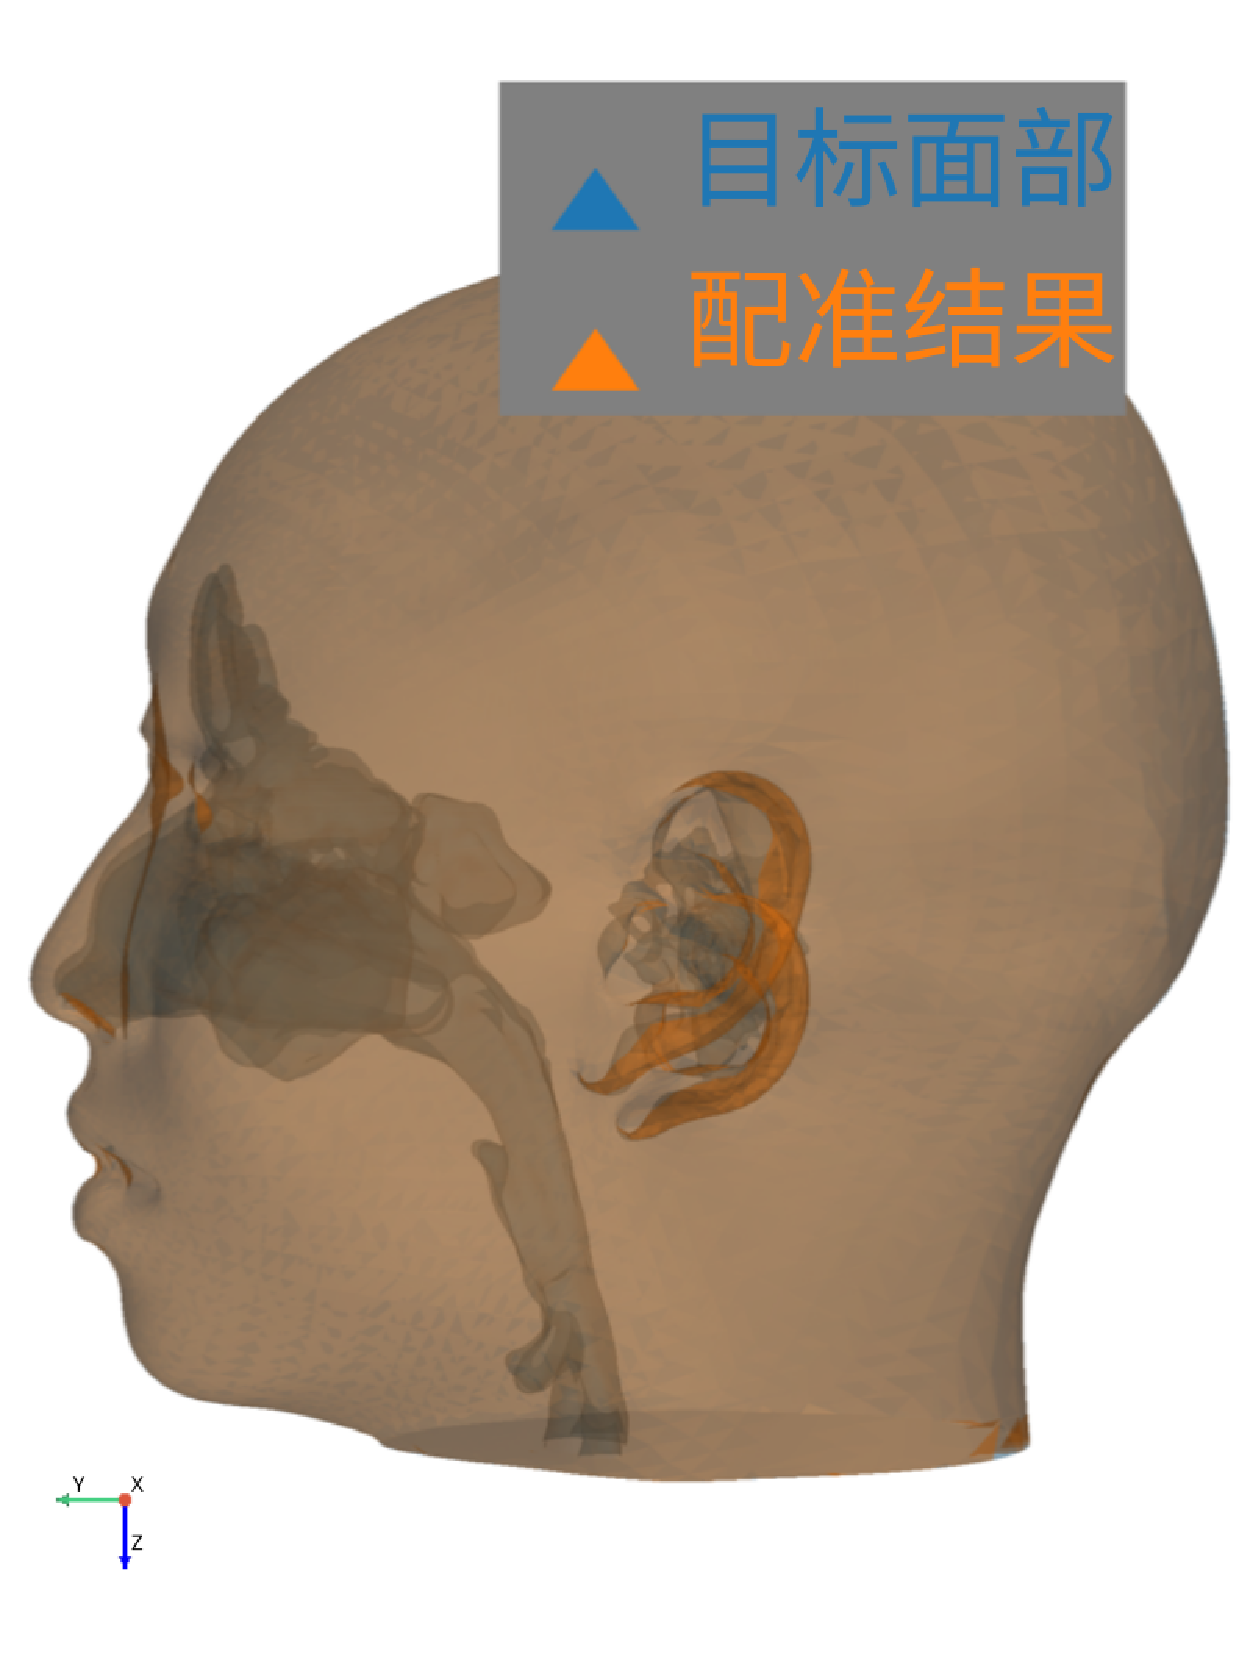
\includegraphics[width = 0.3 \linewidth]{register/register-face.pdf}}
  \subcaptionbox{骨骼}{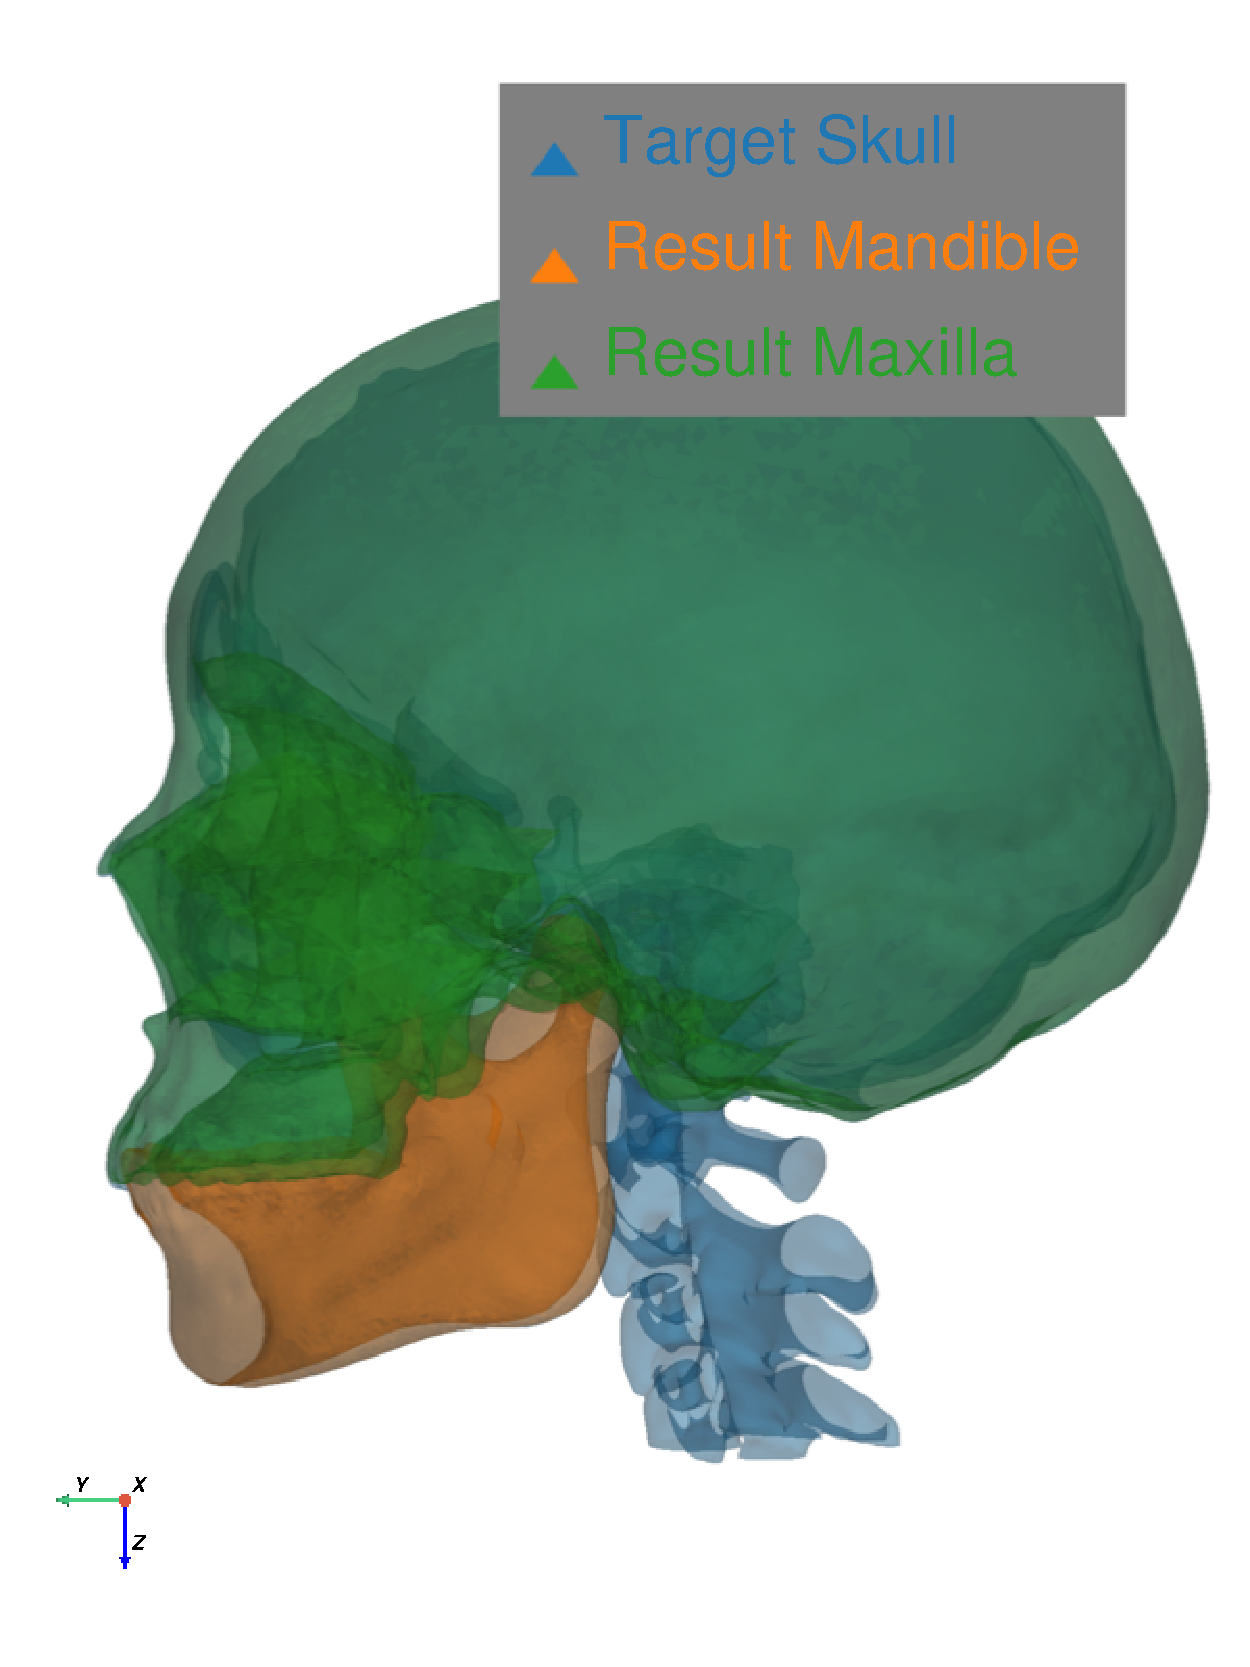
\includegraphics[width = 0.3 \linewidth]{register/register-skull.pdf}}
  \caption{非刚性配准}
  \label{fig:registration}
\end{figure}

\section{四面体网格生成}

在获得模板与患者的三角面网格构型后,我们需将其细分为四面体网格,以适应下一步的仿真分析需求。
在这一过程中,采用了 TetGen 工具 \cite{siTetGenDelaunaybasedQuality2015},其被证实能够生成高品质的四面体网格。
遗憾的是,TetGen 并不能处理含有自相交三角面的输入网格,因此必须对输入模型进行预处理。

我们选用 MeshFix 修复工具 \cite{atteneLightweightApproachRepairing2010},以消除自相交的问题。
修复流程首先独立对面部、上颌骨和下颌骨模型进行处理。
考虑到模板中上下颌骨之间的相交现象,我们将各自修复的结果进行布尔并操作,从而合成一个完整的颅骨模型。
尽管 MeshFix 和布尔操作可能会改变模型的拓扑结构,而不能保证手术前后拓扑结构的一致性,这些变动仅在局部发生。
因此,通过比对手术前和修复后的模型,仍能够识别出拓扑结构保持不变的顶点,利用这些顶点可以追踪手术前后模型之间的对应关系和相应顶点的位移。
至于其余顶点的位移,可通过在 TetGen 所生成四面体网格的骨骼表面插值获得。
鉴于骨骼的刚性特性,我们采用最近邻插值法确保插值结果的准确性。
如图 \ref{fig:tetra} 所示是生成的四面体网格的剖面图。

\begin{figure}
  \centering
  \includegraphics[width = 0.5 \linewidth]{tetra.png}
  \caption{四面体网格剖面}
  \label{fig:tetra}
\end{figure}
